%Copyright 2021 Jean-Michel Bruel
%This program is free template, under the terms of the attached License of this repo. 
%Based on https://github.com/jpeisenbarth/SRS-Tex
%Itself based on the code of Yiannis Lazarides
%http://tex.stackexchange.com/questions/42602/software-requirements-specification-with-latex
%http://tex.stackexchange.com/users/963/yiannis-lazarides
%Also based on the template of Karl E. Wiegers
%http://www.se.rit.edu/~emad/teaching/slides/srs_template_sep14.pdf
%http://karlwiegers.com
\documentclass{scrreprt}
\usepackage{method}		% Specific command from Handbook
\usepackage{minitoc}	% For table of content in chapters
\usepackage{listings}
\usepackage{underscore}
\usepackage{xcolor}
\usepackage{booktabs}
\usepackage{graphicx}
\usepackage{float}
\usepackage[bookmarks=true]{hyperref}
\usepackage[utf8]{inputenc}
\usepackage[english]{babel}
\hypersetup{
    bookmarks=false,    % show bookmarks bar?
    pdftitle={Software Requirement Specification},    % title
    pdfauthor={Jean-Philippe Eisenbarth},                     % author
    pdfsubject={TeX and LaTeX},                        % subject of the document
    pdfkeywords={TeX, LaTeX, graphics, images}, % list of keywords
    colorlinks=true,       % false: boxed links; true: colored links
    linkcolor=blue,       % color of internal links
    citecolor=black,       % color of links to bibliography
    filecolor=black,        % color of file links
    urlcolor=purple,        % color of external links
    linktoc=page            % only page is linked
}%
\def\myversion{1.0.0 }
\date{}
%\title
\usepackage{hyperref}
\newcommand*{\nsection}[1]{
    \section*{#1}
    \addcontentsline{toc}{section}{#1}
}
\newcommand*{\nsubsection}[1]{
    \subsection*{#1}
    \addcontentsline{toc}{section}{#1}
}
%--------------------- Numbering ---------------
\usepackage{amsthm}
\usepackage{xassoccnt}
%\newtheorem{req}{Requirement}[section]        
\newtheorem{req}{Requirement}        
\theoremstyle{definition}        
\newtheorem{constraint}{Constraint}
\newtheorem{goal}{Goal}
\newtheorem{benefit}{Benefit}
\newtheorem{limitation}{Limitation}
\newtheorem{exclusion}{Exclusion}
\DeclareCoupledCountersGroup{theorems}
\DeclareCoupledCounters[name=theorems]{req,constraint,goal}
\setcounter{goal}{0}
%--------------------- Comments ---------------
\newcommand{\mynote}[3][black]{\textcolor{#1}{\fbox{\bfseries\sffamily\scriptsize{#2}}
{\small\textsf{\emph{#3}}}}}
\newcommand{\comment}[1]{\mynote[red]{Comment:}{#1}}
%\newcommand{\comment}[1]{}
\newcommand{\notEmpty}{\comment{This chapter should not be empty!}}

\begin{document}

\begin{center}
    \rule{16cm}{5pt}\vskip1cm
    \begin{bfseries}
        \Huge{SOFTWARE REQUIREMENTS\\ SPECIFICATION}\\
        \vspace{1.9cm}
        Room8\\
        \vspace{1.9cm}
        \LARGE{Version \myversion}\\
        \vspace{1.9cm}
        Prepared by:\\
        Mohammed Abed\\ 
        Maged Armanios\\
        Jinal Kasturiarachchi\\
        Jane Klavir\\
        Harshil Patel\\
        \vspace{0.9cm}
        McMaster University\\
        \vspace{0.9cm}
        \today\\
    \end{bfseries}
\end{center}

%===============================================================
\chapter*{Revision History}
%===============================================================

\begin{center}
    \begin{tabular}{|c|c|c|c|}
        \hline
	    Name        & Date          & Reason For Changes & Version\\
        \hline
        \hline
	    J.-M. Bruel & 2021-01-22    & First Draft & 1.0\\
        \hline
	    J.-M. Bruel & 2023-01-28    & Check after publication of the Handbook & 1.23\\
        \hline
	    J.-M. Bruel & 2023-06-12    & Add reqs automated numbering & 1.23.1 \\
        \hline
	    J.-M. Bruel & 2023-08-25    & Add Minimum Requirements Outcome Principle & 1.23.8 \\
        \hline
	    J.-M. Bruel & 2023-12-22    & Remove section numbers & 1.23.12 \\
        \hline
	    J.-M. Bruel & 2024-08-01    & Add warning about non empty chapters  & \myversion \\
        \hline
    \end{tabular}
\end{center}

This document follows the requirements documentation structure presented in the \href{ https://link.springer.com/content/pdf/10.1007/978-3-031-06739-6.pdf}{Handbook of requirements and business analysis}, by Bertrand Meyer.

%===============================================================
\dominitoc% Initialization
\tableofcontents
\adjustmtc
%===============================================================

%===============================================================
\addcontentsline{toc}{chapter}{Goals book}
\chapter*{Goals}

\minitoc% Creating an actual minitoc
%===============================================================

\comment{Goals are "needs of the target organization, which the system will address". While the development team is the principal user of the other books, the Goals book addresses a wider audience: essentially, all stakeholders.}

\nsection{G.1 Context and overall objective}
%---------------------------------
\begin{flushleft}
Shared living environments often create tension between roommates. It is usually cumbersome to reach out to a roommate about messes they left behind in a shared space, concerns over bill payments, household upkeep, and more. Our project, Room8, aims to prevent these cumbersome interactions by providing an application and the necessary hardware components to help monitor the cleanliness of shared spaces, schedule tasks, track shared billing cycles, and alert roommates of any issues within the shared house.
\end{flushleft}

\begin{goal}\label{goal:first}
Create a system that monitors the cleanliness of a shared living space, such as a kitchen or a living room.
\end{goal}
\begin{goal}\label{goal:second}
Provide roommates with a centralized platform to manage, schedule, and task household tasks.
\end{goal}
\begin{goal}\label{goal:third}
Provide roommates with a centralized platform to manage, schedule, and track bill payments.
\end{goal}
\begin{goal}\label{goal:fourth}
Alert and remind roommates of issues regarding issues related to the shared living spaces, reducing tension between each other.
\end{goal}

\nsection{G.2 Current situation}

\begin{flushleft}
Room8 is designed to reduce points of tension and reduce the need for frustrating dialogue commonplace with people in shared housing, especially students. Currently, in order to manage the many shared responsibilities, roommates have to utilize multiple techniques or tools such as physical calendars, notification reminders, and existing applications such as Splitwise which do not have any integrations between each other. Additionally, it is estimated that approximately 25\% students experience conflicts with a roommate, harming academic performance and inducing stress [1]. Recognizing these factors, Room8 aims to create a centralized platform that not only simplifies communication but reduces stress and conflict to improve the lives of students. 
\end{flushleft}

\nsection{G.3 Expected benefits}
\begin{flushleft}
As stated in section G.2, conflicts between roommates create more than issues in the home and involve more than just misunderstandings in scheduling tasks or living standards. By creating a centralized suite that will help roommates monitor, schedule, and coordinate, Room8 will reduce conflicts between roommates over misunderstandings and miscommunications, and allow for greater flexibility in assigning responsibilities. Additionally, reduced conflicts will lead to mental health benefits for those living in the home by lowering conflict-related stress.  Finally, Room8 is expected to improve academic performance in some students who are hindered academically by conflicts with roommates (approximately 17% of students [1]). 

\begin{benefit}\label{benefit:first}
An improvement in response times amongst roommates over household concerns.
\end{benefit}

\begin{benefit}\label{benefit:first}
Increased flexibility in task scheduling and management, due to the presence of a centralized application.
\end{benefit}

\begin{benefit}\label{benefit:first}
Improved communication and transparency over household matters between roommates.
\end{benefit}

\begin{benefit}\label{benefit:first}
A reduction of events in which a roommate forgets or neglects their responsibilities to the home.
\end{benefit}

\begin{benefit}\label{benefit:first}
Improved household cleanliness and upkeep.
\end{benefit}

\begin{benefit}\label{benefit:first}
A reduction in conflicts between roommates over household matters.
\end{benefit}

\begin{benefit}\label{benefit:first}
A reduction in stress for roommates due to reduced conflicts amongst each other.\end{benefit}

\begin{benefit}\label{benefit:first}
Improved mental health for students who experience conflicts with roommates.
\end{benefit}

\begin{benefit}\label{benefit:first}
An improvement in academic performance for students experience stress caused by issues with roommates.
\end{benefit}

\end{flushleft}

\nsection{G.4 Functionality overview}
\comment{Overview of the functions (behavior) of the system. Principal properties only (details are in the System book).}

\begin{flushleft}
    \item \textbf{User \& House Management:} The system allows students to register, create, and manage their accounts. Students are also able to create homes and invite other students. 
    
    \item \textbf{Cleanliness Management:} Students are able to set up cameras in their shared living spaces. Machine learning algorithms are used to detect messes and assign them to the students to increase accountability and to reduce communication friction. 
    
    \item \textbf{Scheduler:} The system allows users to create and manage chore and cleaning schedules. It will also send reminders to users about their assigned chores and cleaning tasks. Additionally, users are able to "book" common areas that are available within the shared space (i.e. party room, study room, etc.) to avoid conflicts 
     
    \item \textbf{Bill Splitter:} Students are able to add shared expenses to the house and keep track of who owes what. The system will automatically split the bills between the chosen students. 

    \item \textbf{Chat:} The system provides an exportable chatbot to SMS group chats to aid in home management and communication. The chatbot will be able to send remainders and notifications to the group chat about upcoming events, chores, and bills.
    
    \item \textbf{Compliance and Data Privacy:} The system follows data privacy and compliance with Personal Information Protection and Electronic Documents Act (PIPEDA), Ontario’s Freedom of Information and Protection of Privacy Act (FIPPA), and Anti-Spam Legislation (CASL) to ensure that student's data is secure and not shared with third parties.
    
    \item \textbf{Progressive Web App:} The system is hosted as a progressive web app (PWA), so users can use it on their phones and computers.
\end{flushleft}

\nsection{G.5 High-level usage scenarios}
\comment{Fundamental usage paths through the system.}

\begin{figure}[H]
    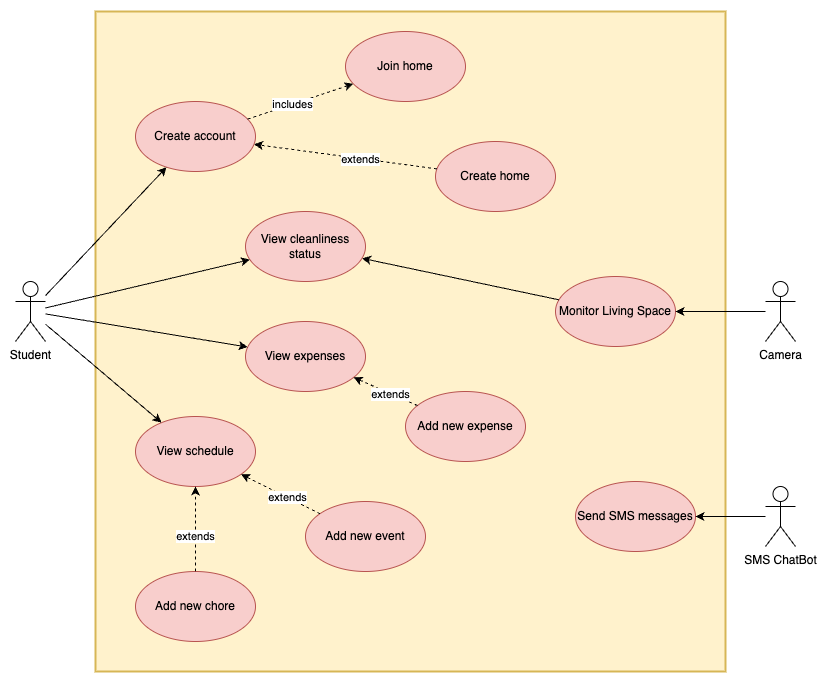
\includegraphics[width=\linewidth]{./img/use-case-diagram.png}
    \caption{High level use case diagram}
    \label{fig: High level use case diagram}
\end{figure}

\begin{itemize}
    \item UC1: Create an account
    \begin{enumerate}
        \item User accesses the Room8 app.
        \item User selects the "Create Account" option.
        \item User fills in personal information (name, email, password).
        \item User submits the form.
        \item System validates the information and creates the account.
        \item System authenticates the user.
        \item System redirects the user to their dashboard.
    \end{enumerate}
    
    \item UC2: Log in to the system
    \begin{enumerate}
        \item User accesses the Room8 app.
        \item User selects the "Log In" option.
        \item User enters email and password.
        \item User submits the form.
        \item System authenticates the credentials and logs in the user.
        \item System redirects the user to their dashboard.
    \end{enumerate}
    
    \item UC3: Log out of the system
    \begin{enumerate}
        \item User accesses the main menu of the Room8 app.
        \item User selects the "Log Out" option.
        \item System prompts for confirmation.
        \item User confirms the action.
        \item System logs the user out and redirects to the login screen.
    \end{enumerate}
    
    \item UC4: Create a home
    \begin{enumerate}
        \item User navigates to their dashboard.
        \item User selects the "Create Home" option.
        \item User enters home details (home name, address, etc.).
        \item User sends invitations to housemates by entering their email addresses.
        \item System sends email notifications to invited users.
        \item Invited users accept or decline the invitation.
    \end{enumerate}
    
    \item UC5: Join a home
    \begin{enumerate}
        \item User receives an email invitation to join a home.
        \item User clicks on the provided link in the invitation.
        \item System redirects user to the Room8 app.
        \item User logs in or creates an account if not logged in.
        \item User confirms their decision to join the home.
        \item System adds the user to the home group.
    \end{enumerate}
    
    \item UC6: Leave a home
    \begin{enumerate}
        \item User navigates to their Home settings.
        \item User chooses the "Leave Home" option.
        \item System prompts for confirmation.
        \item User confirms the action.
        \item System removes the user from the home group.
    \end{enumerate}
    
    \item UC7: Update user profile
    \begin{enumerate}
        \item User navigates to the “Profile” section.
        \item User selects the "Edit Profile" option.
        \item User modifies personal information (name, profile picture, etc.).
        \item User saves changes.
        \item System updates the user’s profile information.
    \end{enumerate}
    
    \item UC8: Schedule a chore
    \begin{enumerate}
        \item User navigates to the "Schedule” section.
        \item User selects "Add New Chore".
        \item User inputs chore details (name, description, time, frequency, assigned users, etc.).
        \item System saves the chore and sends reminders to the assigned users.
    \end{enumerate}
    
    \item UC9: Edit a chore
    \begin{enumerate}
        \item User navigates to the "Schedule” section.
        \item User selects a scheduled chore.
        \item User chooses the "Edit" option.
        \item User modifies the chore details (name, description, time, frequency, assigned users, etc.).
        \item System updates the chore and notifies relevant housemates.
    \end{enumerate}
    
    \item UC10: Complete a chore
    \begin{enumerate}
        \item User navigates to the "Schedule” section.
        \item User selects a chore assigned to them.
        \item User chooses the "Complete" option.
        \item System marks the chore as complete and updates the chore history.
    \end{enumerate}
    
    \item UC11: Add event to schedule
    \begin{enumerate}
        \item User navigates to the "Schedule" section.
        \item User selects the "Add Event" option.
        \item User inputs event details (date, time, description).
        \item User sets reminders or notifications if needed.
        \item System adds the event to the users' schedule.
    \end{enumerate}
    
    \item UC12: View chore history
    \begin{enumerate}
        \item User navigates to the "Schedule” section.
        \item User selects the "Chore History" option.
        \item System displays a list of completed and pending chores.
        \item User can filter or search through the history.
    \end{enumerate}
    
    \item UC13: Add an expense
    \begin{enumerate}
        \item User navigates to the “Bill Splitter” section.
        \item User selects the "Add Expense" option.
        \item User enters the total expense amount and description.
        \item User selects which housemates are responsible for the expense.
        \item System splits the expense and notifies the involved users.
    \end{enumerate}
    
    \item UC14: Edit an expense
    \begin{enumerate}
        \item User navigates to the “Bill Splitter” section.
        \item User selects an expense to edit.
        \item User modifies the expense details (amount, description, responsible users).
        \item System updates the expense and notifies the involved users.
    \end{enumerate}
    
    \item UC15: Pay an expense
    \begin{enumerate}
        \item User navigates to the "Bill Splitter" section.
        \item User selects their profile's bills.
        \item User selects an unpaid bill.
        \item User marks the bill as paid.
        \item System updates the payment status.
        \item System notifies other housemates about the payment status.
    \end{enumerate}
    
    \item UC16: View expense history
    \begin{enumerate}
        \item User navigates to the "Bill Splitter" section.
        \item User selects the "Expense History" option.
        \item System displays a list of past payments and outstanding bills.
        \item User can filter the history by type or amount.
    \end{enumerate}
    
    \item UC17: View current cleanliness status
    \begin{enumerate}
        \item User navigates to the “Cleanliness Management” section.
        \item System displays the current cleanliness score and detected messes.
        \item User selects another user to view their cleanliness score.
        \item System displays the selected user’s cleanliness score and pending tasks.
    \end{enumerate}
    
    \item UC18: View cleanliness history
    \begin{enumerate}
        \item User navigates to the “Cleanliness Management" section.
        \item User selects the "Cleanliness History" option.
        \item System displays a list of detected messes and cleanliness scores over time.
        \item User can filter the history by location or date.
    \end{enumerate}
    
    \item UC19: Add chatbot to group chat
    \begin{enumerate}
        \item User navigates to the “Chat Management” section.
        \item User selects the option to add a chatbot to their house group chat.
        \item User inputs notification and reminder settings.
        \item System generates an SMS numbers and instructions to add the chatbot to the group chat.
        \item The chatbot sends a welcome message to the group.
    \end{enumerate}
    
    \item UC20: Edit chatbot settings
    \begin{enumerate}
        \item User navigates to the “Chat Management” section.
        \item User selects the "Chatbot Settings" option.
        \item User configures the chatbot’s behavior (e.g., reminders, notifications).
        \item User saves the settings.
        \item System updates the chatbot based on the new settings.
    \end{enumerate}
    
\end{itemize}
    
\nsection{G.6 Limitations and exclusions}
\comment{Aspects that the system need not address.}
Below is a list of limitations and exclusions the system will not address:
\begin{limitation}\label{limitation:first}
System will not track activity completed by the user in the shared environment.
\end{limitation}
\begin{exclusion}\label{exclusion:first}
System will not request or send money directly to users in the bill splitting functionality.
\end{exclusion}
\begin{exclusion}\label{exclusion:second}
System will not use images taken to train machine learning model.
\end{exclusion}

\nsection{G.7 Stakeholders and requirements sources}
\comment{Groups of people who can affect the project or be affected by it, and other places to consider for information about the project and system.}
%---------------------------------
\notEmpty{}
%---------------------------------

\begin{table}[ht]
\centering
\begin{tabular}{|l|l|}
\hline
\textbf{Stakeholder} & \textbf{Category} \\ \hline
Students              & Direct  \\ \hline
Home Managers         & Indirect \\ \hline
University Housing and Social Committee & Indirect \\ \hline
\end{tabular}
\caption{Stakeholders and Categories}
\end{table}

\nsubsection{G.7.1 Direct Stakeholders}
\textbf{Students} \\ Students are the primary direct stakeholders for Room8. They are the main users of the mobile application who create houses within the app and set up the camera systems. These students seek to maintain cleanliness in their shared living spaces and establish accountability when a mess is left behind by a roommate. The application addresses common challenges faced by students in shared living arrangements, such as maintaining cleanliness, splitting expenses, and scheduling activities. 

\nsubsection{G.7.2 Indirect Stakeholders}
\textbf{Home Managers} \\ Home managers are indirect stakeholders to the project. Home managers includes landlords renting out their homes to students or residence assistants managing a room of students. The home managers look to maintain the clean condition of the shared space which is done by holding students accountable for messes that are made. 
\\
\\
\textbf{University Housing and Social Committee} \\ The University Housing and Social Committee is another key indirect stakeholder in the project. These committees often seek to help students transition into living in shared spaces and provide guidance and support. Room8 offers a wide range of services that address common points of frustration faced by students, which are often brought up to these university committees. By facilitating better communication and organization, Room8 helps enhance the overall living experience for students.



%===============================================================
\chapter*{Environment}
\addcontentsline{toc}{chapter}{Environment book}
\minitoc% Creating an actual minitoc
%===============================================================

\comment{The Environment book describes the application domain and external context, physical or virtual (or a mix), in which the system will operate.}

\nsection{E.1 Glossary}
\comment{Clear and precise definitions of all the vocabulary specific to the application domain, including technical terms, words from ordinary language used in a special meaning, and acronyms.
This chapter should not be empty!}

\nsection{E.2 Components}
\comment{List of elements of the environment that may affect or be affected by the system and project. Includes other systems to which the system must be interfaced.}
\begin{flushleft}
  \item \textbf{Motion-activated camera:} The app will be connected to a camera that is activated by motion in the shared space. This component is used for taking a “before” and “after” picture that serves as the input for the cleanliness detection model. \newline
  
  \item \textbf{Object detector API:} The app will utilize an object detector that performs on a pair of images (i.e. the “before” and “after” picture) taken by the motion-activated camera. Object detection enables the algorithm to quantify the difference in room states as a function of objects and their transformations.\newline 
  
  \item \textbf{Household items dataset:} The ML model will be pre-trained with a dataset containing common household and kitchen items. This will allow the object detector to classify the items it detects and is important for providing valuable output to students.\newline
   
  \item \textbf{Google calendar API:} The application will interface with Google calendar to facilitate scheduling chores and events. This is critical for Room8's chore scheduling.\newline

  \item \textbf{SMS Chatbot:} The application employs a chatbot to send notifications to students via SMS about their responsibilities in the home (i.e. cleaning their mess from shared spaces, upcoming chore deadlines, and money owed for shared bills). This helps with bookkeeping, enforcing fairness, and keeping shared spaces clean.\newline

  \item \textbf{OAuth 2.0:}The app utilizes the OAuth 2.0 protocol to manage user authentication and authorization securely. OAuth 2.0 allows Room8 to provide a seamless login experience using third-party identity providers without requiring users to create and manage separate credentials. OAuth 2.0 handles the app’s legal and privacy compliance standards.\newline

\end{flushleft}

\nsection{E.3 Constraints}
\comment{Obligations and limits imposed on the project and system by the environment.}
%---------------------------------
\begin{flushleft}
  \item \textbf{Camera resolution:} The resolution of the motion-activated camera affects the quality of the input that is used by the object detector. Depending on the PPM of the image, there is a minimum viable object size for a given object to be classified.\newline
  
  \item \textbf{Platform compatibility:} The application must be compatible on Android and iOS to accommodate all users in the home.\newline 
  
  \item \textbf{Data privacy compliance:} The application adheres to all applicable data privacy regulations for the region in which it operates. User data must be handled with the utmost care and cannot be shared or used without explicit consent. Prior to collecting, storing, or processing any personal data, the appropriate permissions must always be obtained to ensure compliance with privacy laws and to respect user rights. \newline

\end{flushleft}
%---------------------------------


\nsection{E.4 Assumptions}
\comment{Properties of the environment that may be assumed, with the goal of facilitating the project and simplifying the system.}
\begin{flushleft}
  \item \textbf{Network connectivity:} The application assumes that there is reliable internet connection. Operating under this assumption, the camera is able to transfer images to the detector and users have access to updated synchronized information when using the app.\newline

  \item \textbf{Operating system support:} The application is compatible with the versions of Android and iOS that are currently supported by mobile providers.\newline
  
  \item \textbf{Common household items dataset:} The classifier can assume that any object it comes across is a common household item that belongs to a class represented in its training data.\newline 

\end{flushleft}
\nsection{E.5 Effects}
\comment{Elements and properties of the environment that the system will affect.}
\begin{flushleft}
  \item \textbf{Digital minimalism:} Members of the home conduct all interactions on one platform. All common virtual services are provided by the Room8 application, hence eliminating the need for other applications that clutter the digital space.\newline

  \item \textbf{Accountability:} The application promotes social responsibility and user accountability by assessing the cleanliness state of the room before/after use and quantifying the difference in the 2 states. Students are given objective feedback on how their usage of the room contributed to cleanliness and all students in the group are held accountable for their usage.\newline
  
  \item \textbf{Ease social tension:} Students living in a home can feel tense about confronting their roommates when asking them to clean up, pay them back, or do the chores they agreed to. The chatbot sends reminders about these duties, taking the pressure off students to confront each other and risk compromising their relationships.\newline 
\end{flushleft}

\nsection{E.6 Invariants}
\comment{Properties of the environment that the system’s operation must preserve.}

%===============================================================
\chapter*{System}
\addcontentsline{toc}{chapter}{System book}
\minitoc% Creating an actual minitoc
%===============================================================

\comment{The System book refines the Goal one by focusing on more detailed requirements about the system under development, mainly its constituents, behaviors and properties.}

\nsection{S.1 Components}
\comment{Overall structure expressed by the list of major software and, if applicable, hardware parts.}
%---------------------------------
\notEmpty{}
%---------------------------------
\begin{figure}[H]
    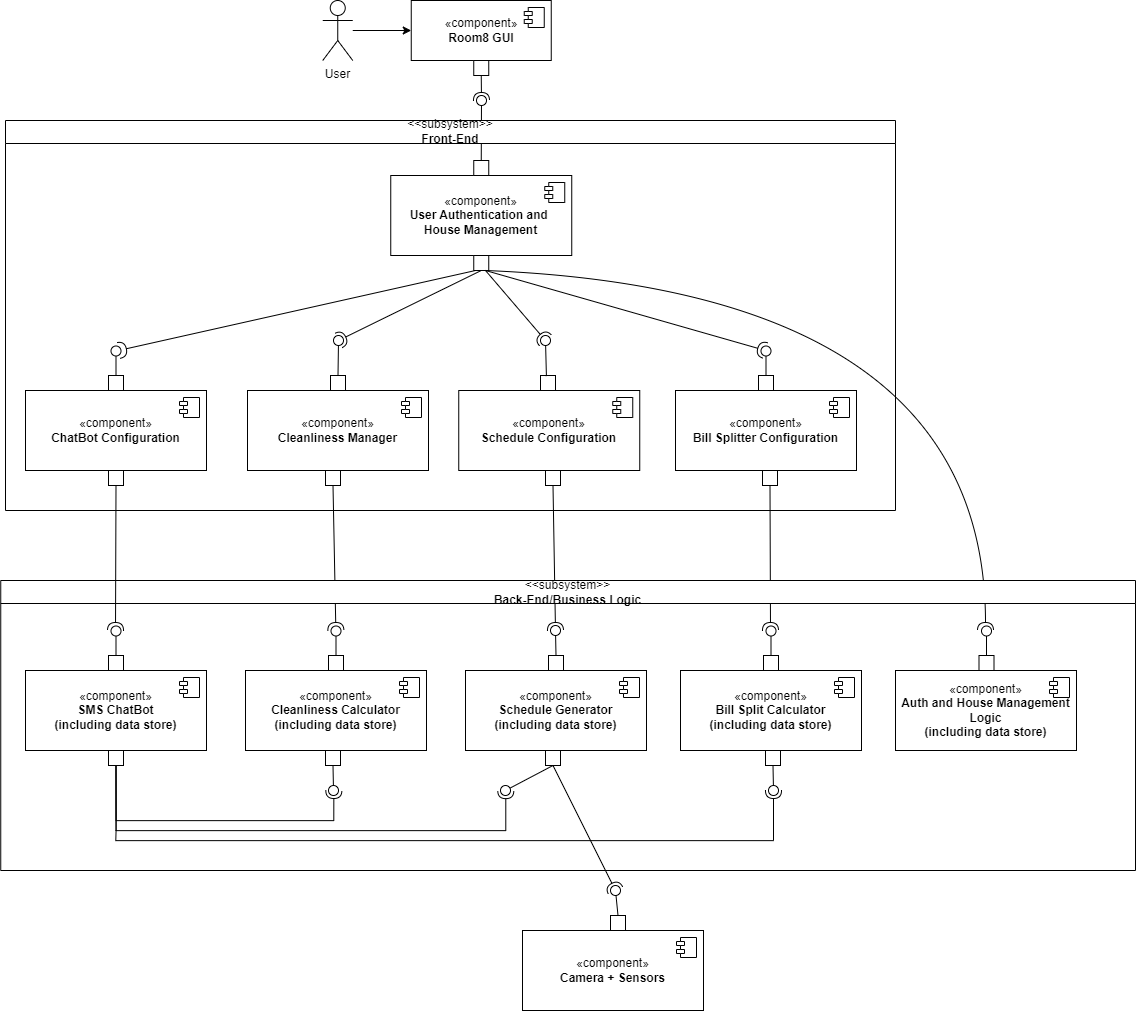
\includegraphics[width=\linewidth]{./img/component-diagram.png}
    \caption{Component Diagram}
    \label{fig: High level component diagram}
\end{figure}

\nsection{S.2 Functionality}
\comment{One section, S.2.n, for each of the components identified in S.2, describing the corresponding behaviors (functional and non-functional properties).}
%---------------------------------
\notEmpty{}
%---------------------------------

\nsection{S.3 Interfaces}
\comment{How the system makes the functionality of S.2 available to the rest of the world, particularly user interfaces and program interfaces (APIs).}

\nsection{S.4 Detailed usage scenarios}
\comment{Examples of interaction between the environment (or human users) and the system: use cases, user stories.}

\nsection{S.5 Prioritization}
\comment{Classification of the behaviors, interfaces and scenarios (S.2, S.3 and S.4) by their degree of criticality.}

\nsection{S.6 Verification and acceptance criteria}
\comment{Specification of the conditions under which an implementation will be deemed satisfactory.}

%===============================================================
\chapter*{Project}
\addcontentsline{toc}{chapter}{Project book}
\minitoc% Creating an actual minitoc
%===============================================================

\comment{The Project book describes all the constraints and expectations not about the system itself, but about how to develop and produce it.}

\nsection{P.1 Roles and personnel}
\comment{Main responsibilities in the project; required project staff and their needed qualifications.}

\nsection{P.2 Imposed technical choices}
\comment{Any a priori choices binding the project to specific tools, hardware, languages or other technical parameters.}

\nsection{P.3 Schedule and milestones}
\begin{itemize}
    \item \textbf{Milestone 1 (September 23rd) - Initial concept and development plan}
    \begin{itemize}
        \item Deliverable: Problem Statement and Goals
        \item Deliverable: Development Plan
    \end{itemize}

    \item \textbf{Milestone 2 (October 11) - Requirements}
    \begin{itemize}
        \item Deliverable: SRS
    \end{itemize}

    \item \textbf{Milestone 3 (October 23) - Hazard Analysis}
    \begin{itemize}
        \item Deliverable: Hazard Analysis Report
    \end{itemize}

    \item \textbf{Milestone 4 (November 1st) - V\&V Plan}
    \begin{itemize}
        \item Deliverable: V\&V Plan
    \end{itemize}

    \item \textbf{Milestone 5 (Within November 11-22) - POC demonstration}
    \begin{itemize}
        \item Event: Informal Project Demonstration
        \item Goal: Core features functional
    \end{itemize}

    \item \textbf{Milestone 6 (January 15) - Design Documents}
    \begin{itemize}
        \item Deliverable: Software Architecture Document
        \item Deliverable: Detailed Design Document
    \end{itemize}

    \item \textbf{Milestone 7 (within February 3-14) - Revision 0 \& Project completion}
    \begin{itemize}
        \item Goal: Project is Complete and Functional
    \end{itemize}

    \item \textbf{Milestone 8 (March 7th) - Verify \& Validate}
    \begin{itemize}
        \item Deliverable: V\&V Report
        \item Goal: Project meets all requirements outlined in the SRS and V\&V Plan
    \end{itemize}

    \item \textbf{Milestone 9 (within March 24-30) - Final demonstration}
    \begin{itemize}
    	\item Event: Final Project Demonstration
    	\item Goal: Unmet requirements from Milestone 8 are resolved
    \end{itemize}

    \item \textbf{Milestone 10 (April) - Project EXPO demonstration}
    \begin{itemize}
        \item Deliverable: Project Poster
        \item Event: Project Expo
    \end{itemize}

    \item \textbf{Milestone 11 (April 2nd) - Final documentation}
    \begin{itemize}
        \item Deliverable: Final Problem Statement
        \item Deliverable: Development Plan
        \item Deliverable: POC Plan
        \item Deliverable: Updated Requirements document
        \item Deliverable: V\&V Plan
        \item Deliverable: V\&V Report
        \item Deliverable: User Guide
        \item Deliverable: Project Source Code
    \end{itemize}
\end{itemize}

\nsection{P.4 Tasks and deliverables}
\comment{Details of individual tasks listed under P.3 and their expected outcomes.}
%---------------------------------
\notEmpty{}
%---------------------------------

\nsection{P.5 Required technology elements}
\comment{External systems, hardware and software, expected to be necessary for building the system.}\\
\textbf{Camera} \\
A camera is used for the systems cleanliness detection aspect. A camera takes pictures for comparing the state of the shared space.\\
\\
\textbf{Motion Sensor}\\
A sensor is also used for the systems cleanliness detection aspect. The sensor detects movement which will work in unison with the camera to take pictures of the shared space.\\
\\
\textbf{Google Calendar API}\\
Room8's scheduler requires a calendar component where user's can book and view events and chores in a calendar Google's Calendar API.\\
\\
\textbf{Secure Database}\\
Users create accounts for Room8 where user and home information is stored on a secure database where sensitive information such as credentials are stored and individuals are able to change and delete accounts.\\
\\
\textbf{Gmail OAuth}\\
Users will sign in securely without risk of data leaks and malicious connections.\\
\\
\textbf{SMS Message Service}\\
Room8's Chatbot SMS will send messages to users using a third party messaging system that has connection to the Room8 application to send warnings and information of shared space.\\


\nsection{P.6 Risks and mitigation analysis}
\comment{Potential obstacles to meeting the schedule of P.4, and measures for adapting the plan if they do arise.}\\
\textbf{Machine Learning Model Training}\\
Finding enough data to train the machine learning algorithm to detect when a mess has been made and what detect what is altered or added in the space. Sensitivity to slight changes such as lighting is another risk with the machine learning algorithm approach. An alternative to adapt this scenario would be to use image differencing to detect changes in environment.\\
\\
\textbf{User Identification}\\
Being able to detect which user is using the shared space through the camera is a major risk. The program may not be supplied with enough information to identity which user is currently using the space. In order to work around this the program could get individuals to submit to the application that they are now using the space.\\
\\
\textbf{Scope Creep}\\
Unclear requirements and adding too many elements to the scope of the project will result in not delivering on features that are listed to be part of the application and lower quality of core functionality due to time being strain. A revisal of requirements by making requirements and functionality of system clear and concise and developing a prioritization list would mitigate the risk of scope creep.


\nsection{P.7 Requirements process and report}
\comment{Initially, description of what the requirements process will be; later, report on its steps.}

\newpage{}
\section*{Appendix --- Reflection}

The information in this section will be used to evaluate the team members on the
graduate attribute of Lifelong Learning.  

% The purpose of reflection questions is to give you a chance to assess your own
learning and that of your group as a whole, and to find ways to improve in the
future. Reflection is an important part of the learning process.  Reflection is
also an essential component of a successful software development process.  

Reflections are most interesting and useful when they're honest, even if the
stories they tell are imperfect. You will be marked based on your depth of
thought and analysis, and not based on the content of the reflections
themselves. Thus, for full marks we encourage you to answer openly and honestly
and to avoid simply writing ``what you think the evaluator wants to hear.''

Please answer the following questions.  Some questions can be answered on the
team level, but where appropriate, each team member should write their own
response:


\begin{enumerate}
  \item What went well while writing this deliverable? 
  \item What pain points did you experience during this deliverable, and how did
  you resolve them?
  \item How many of your requirements were inspired by speaking to your
  client(s) or their proxies (e.g. your peers, stakeholders, potential users)?
  \item Which of the courses you have taken, or are currently taking, will help
  your team to be successful with your capstone project.
  \item What knowledge and skills will the team collectively need to acquire to
  successfully complete this capstone project?  Examples of possible knowledge
  to acquire include domain specific knowledge from the domain of your
  application, or software engineering knowledge, mechatronics knowledge or
  computer science knowledge.  Skills may be related to technology, or writing,
  or presentation, or team management, etc.  You should look to identify at
  least one item for each team member.
  \item For each of the knowledge areas and skills identified in the previous
  question, what are at least two approaches to acquiring the knowledge or
  mastering the skill?  Of the identified approaches, which will each team
  member pursue, and why did they make this choice?
\end{enumerate}


%===============================================================
\end{document}
%===============================================================